\label{sec:characteristics}
A meteoroid in our model is described with a number of features before it starts descending through the atmosphere.
It has a mass, a velocity, a density, a trajectory angle relative to the planetary surface, and a strength that indicates how much aerodynamic stress it can withstand before breaking up into pieces. 

In a survey of 77 recent impact crater clusters on Mars, \cite{daubar2019recently} studied a number of characteristics of these clusters.
In the following work, we investigate whether these characteristics allow us to constrain the range of possible values for the meteoroid features; e.g., whether we can constrain the mass of the meteoroid based on a combination of these characteristics.

Because of the limited scope of this project, we had to make a handful of arbitrary choices about the variant of our model to use.
Our choices were largely based on the work by \cite{newland2019CFM18}. They used the fragment-cloud model (sec.~\ref{sec:fragment_cloud_model}) with random fragment mass fractions, but without the random element to strength scaling (cf. sec.~\ref{sec:fragments_model}).
\cite{newland2019CFM18} also made use of the 2018 extension to the fragment-cloud model that specifies an inner meteoroid structure.
Based on the results presented in \cite{wheeler2018atmospheric}, \cite{newland2019CFM18} defined a simplified inner structure outlined in table~\ref{tab:eric_inner_structure}.
Three structural groups are specified, all making up one third of the total meteoroid mass.
At first break up, the meteoroid will split into 13 pieces, in total, of varying size.
The smaller pieces have a considerably smaller strength $\sigma_b$ compared to the largest piece with a strength of $\sigma_c$. The medium size pieces of the second group are in between.
This reflects the findings by \cite{wheeler2018atmospheric}, who found that in their simulations, best agreement with the data was achieved if, in general, the larger pieces in their inner structure had a higher strength.
Assuming this inner structure, \cite{newland2019CFM18} were able to produce a distribution of certain cluster characteristics that was similar to the clusters presented in the \cite{daubar2019recently} survey. Such a good match to observation was not possible when a homogeneous inner structure was used.
This model is therefore a good starting point for our study.

\begin{table}[htbp]
    \centering
    \begin{tabular}{r|ccc}
        mass fraction (\%) & & $1/3$ \\
        pieces & $1$ & $3$ & $9$ \\
        strength & $\sigma_c$ & $\sqrt{\sigma_c\sigma_b}$ & $\sigma_b$ \\
        Weibull exponent & & $0.25$ \\
        cloud mass fraction & & $0.5$ \\
        frag. mass fractions & \multicolumn{3}{c}{$(0.05 - 0.5$, $0.5 - 0.95)$}
    \end{tabular}
    \caption{Meteoroid inner structure proposed by \cite{newland2019CFM18}, based on results from \cite{wheeler2018atmospheric}. For the Weibull exponent and the cloud mass fraction, we chose a fixed value based on the average used in \cite{wheeler2018atmospheric}.}
    \label{tab:eric_inner_structure}
\end{table}

The characteristics studied by \cite{daubar2019recently} and \cite{newland2019CFM18} are listed in table~\ref{tab:charcteristics}. For each of these, we studied (a) how variable they are for a given meteoroid as a result of randomness in the breakup process, and (b) how well they constrain the range of possible meteoroid features.
For (a), we defined a set of meteoroid features that is representative of the space of possible values.
Then we repeated the same simulation with different seeds to the random number generator (RNG) and computed the crater characteristics. Two examples are displayed in figures \ref{fig:characteristics_variability_1} and \ref{fig:characteristics_variability_2}.
For (b), we ran a Monte-Carlo simulation across the entire range of meteoroid features that would lead to a cluster with effective diameter between about $1\,\mathrm{m}$ and $50\,\mathrm{m}$.
Parameters for both parts are listed in table~\ref{tab:mc_params}.

\begin{figure*}
    \centering
    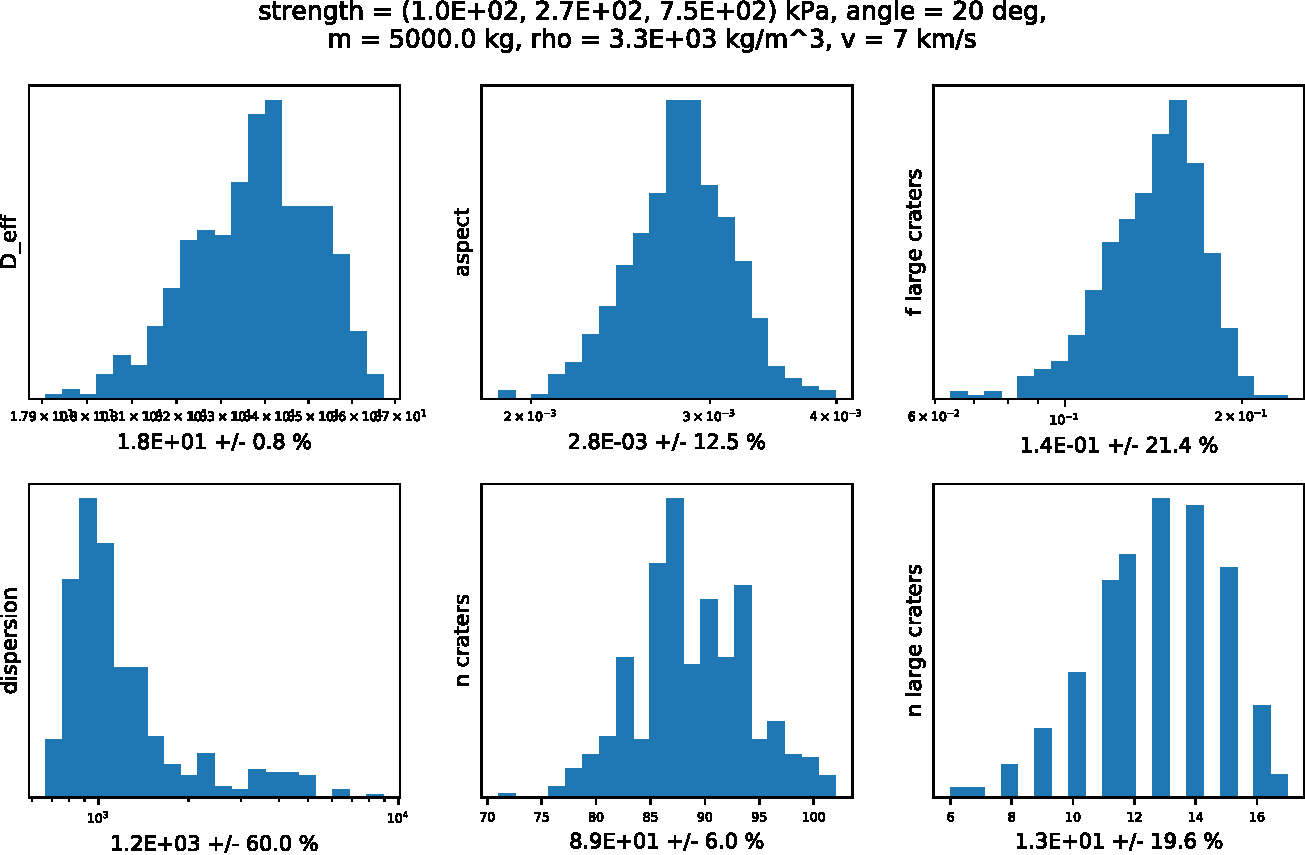
\includegraphics[width=\textwidth]{figures/crater_tools_analysis_1}
    \caption{Crater characteristics computed from running the forward model with parameters in the title and 500 different seeds for the random number generator.}
    \label{fig:characteristics_variability_1}
\end{figure*}

\begin{figure*}
    \centering
    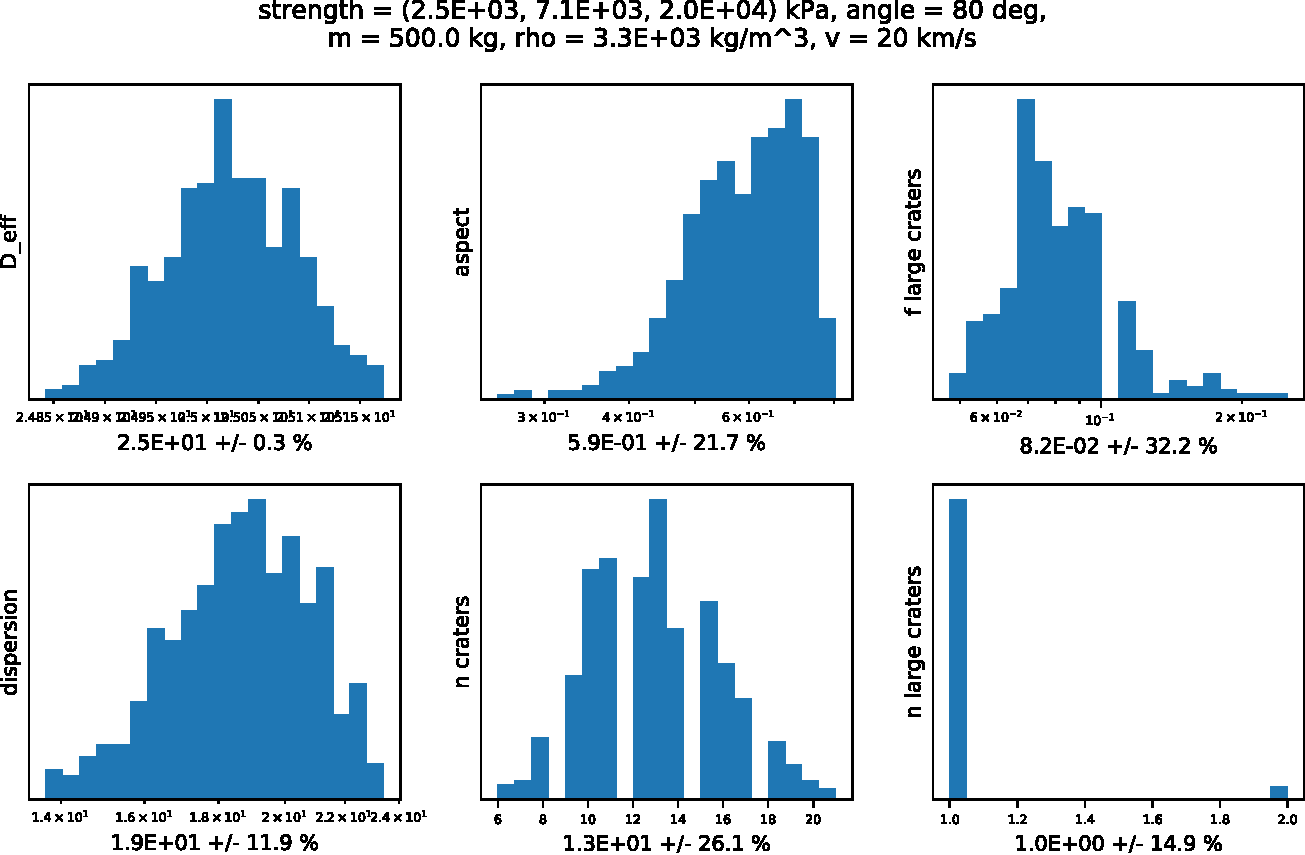
\includegraphics[width=\textwidth]{figures/crater_tools_analysis_2}
    \caption{Crater characteristics computed from running the forward model with the same parameters in the title 500 different seeds for the random number generator.}
    \label{fig:characteristics_variability_2}
\end{figure*}

\begin{table}[htbp]
    \centering
    \begin{tabular}{l|l}
        effective diameter & $\left(\sum_i d_i^3\right)^{1/3}$, $d_i$ the \\ & crater diameters \\[0.4em]
        aspect ratio & ratio of minor to major \\ & axis of best fit ellipse \\ & around the cluster \\[0.4em]
        dispersion & median distance \\ & between craters \\[0.4em]
        $n$ craters & number of craters \\ & in a cluster \\[0.4em]
        $f$ large craters & fraction of craters \\ & larger than a threshold
    \end{tabular}
    \caption{Crater characteristics studied by \cite{daubar2019recently} and/or \cite{newland2019CFM18}.}
    \label{tab:charcteristics}
\end{table}

\begin{table*}
    \centering
    \begin{tabular}{l|l l}
        & \multicolumn{1}{c}{(a)} & \multicolumn{1}{c}{(b)} \\
        \hline
        mass $m$ (kg) & $\log(m) \sim \mathcal{U}[\log(0.1),\, \log(2\e{4})]$ & $m \in \{0.3, 500, 500 \}\unit{kg}$ \\
        density $\rho$ & \multicolumn{2}{c}{$\rho = 3330 \unit{\frac{kg}{m^3}}$} \\
        velocity $v$ (km/s) & $\log(v) \sim \mathcal{U}[\log(6),\, \log(30)]$ & $v \in \{7, 12, 20\} \unit{\frac{km}{s}}$ \\
        bulk strength $\sigma_b$ (kPa) & $\log(\sigma_b) \sim \mathcal{U}[\log(1),\, \log(10^5)]$ & $\sigma_b \in \{100, 500, 2500\} \unit{kPa}$ \\
        core strength $\sigma_c$ (kPa) & $\log(\sigma_c) \sim \mathcal{U}[\log(\sigma_b),\, \log(10^5)]$ & $\sigma_c \in \{750, 4000, 2\e{4}\} \unit{kPa}$ \\
        angle $\theta$ (deg) & $\log(\theta) \sim \mathcal{U}[\log(10),\, \log(90)]$ & $\theta \in \{20, 45, 80\}\unit{deg}$
    \end{tabular}
    \caption{Meteoroid features used for the Monte-Carlo studies in section~\ref{sec:characteristics}. $x\sim\mathcal{U}[a, b]$ means that the value $x$ is drawn from a uniform distribution in the interval $[a, b]$. For $\theta < 10\unit{deg}$, the meteoroid almost always either escaped the atmosphere again in our simulation or did not produce detectable craters.}
    \label{tab:mc_params}
\end{table*}

\subsection{Effective diameter}
The effective diameter $D_\mathrm{eff}$ of a crater cluster is a measure of the total volume of all craters. A common assumption is that it is a good proxy for the impactor mass (citation needed).
Figure~\ref{fig:d_eff_vs_m} shows that the relationship is a bit more complicated. We can infer that for our model, $D_\mathrm{eff}$ provides a lower bound for the meteoroid mass, but that the spread of meteoroid masses that can produce clusters of the same $D_\mathrm{eff}$ is quite wide.
Fig.~\ref{fig:d_eff_vs_m} is colour coded by the trajectory angle $\theta$. It shows that a shallower angle increases the lower bound for the mass significantly.
At a given angle, most samples are within a band close to the lower bound, except for a number of outliers. The outliers mostly occur for weak meteoroids.

\begin{figure*}
    \centering
    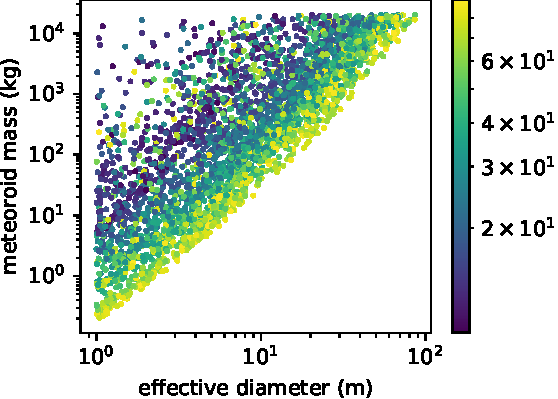
\includegraphics[width=0.45\textwidth]{figures/d_eff_vs_mass}
    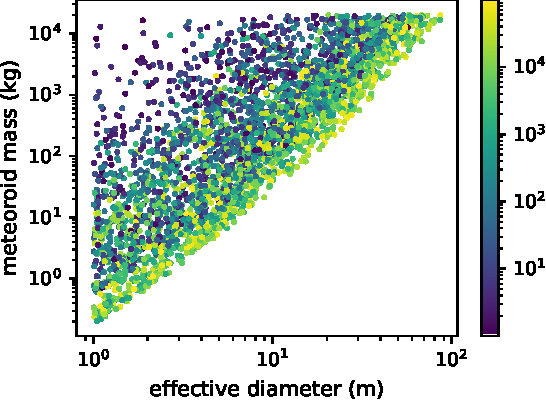
\includegraphics[width=0.45\textwidth]{figures/d_eff_vs_mass_strength}
    \caption{Effective diameter vs initial meteoroid mass. Left colour = initial trajectory angle in degrees from horizontal. Right colour = core strength $\sigma_c$. We can see that at a given angle, mass and effective diameter are highly correlated. Similarly for a given strength.}
    \label{fig:d_eff_vs_m}
\end{figure*}

$D_\mathrm{eff}$ also provides useful information about the strength of the largest piece ($\sigma_c$ in tab.~\ref{tab:eric_inner_structure}) in our inner structure. Figure~\ref{fig:d_eff_vs_strength} shows that at a given meteoroid mass, there is an upper limit to the effective diameter that the cluster can have, and that this limit increases for higher core strengths.
The same pattern cannot be observed for the strengths of the other structural groups. This is probably because the effective diameter is dominated by the largest craters produced by the largest pieces, which will be produced by fragments of the strongest group.

\begin{figure}[htbp]
    \centering
    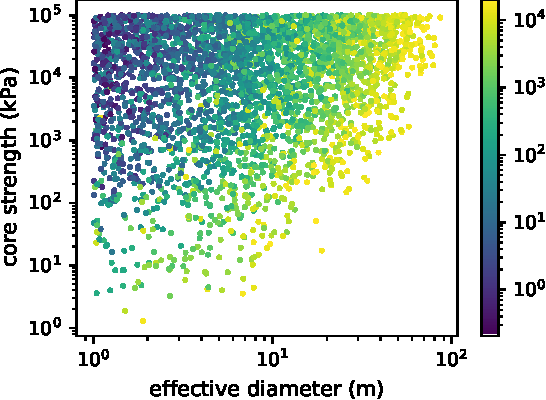
\includegraphics[width=0.45\textwidth]{figures/d_eff_vs_strength}
    \caption{Effective diameter vs. core strength ($\sigma_c$ in tab.~\ref{tab:eric_inner_structure}). The colour code corresponds to the meteoroid mass in kg. We can see that at a given mass, $\sigma_c$ and effective diameter are correlated.}
    \label{fig:d_eff_vs_strength}
\end{figure}

Overall, we conclude that $D_\mathrm{eff}$ provides useful information about the meteoroid mass and strength, and constrains the most likely values even better if other measures are taken into account that restrict the trajectory angle and meteoroid strength. The analysis with variable RNG seeds shows that it is by far the most stable characteristic out of the ones we considered. The relative variability is of the order of $1 - 2\%$ in all scenarios that we looked at.

\subsection{Aspect ratio}
The aspect ratio is defined as the ratio of the semi-minor and semi-major axis of the ellipse with the smallest area that envelops all craters in a cluster.
It was proposed in the \cite{daubar2019recently} survey as a proxy for the initial trajectory angle $\theta$. 
There are several ways to compute this ratio. In this study, we use principal component analysis (PCA).
The ratio of variances explained by the two principal components is equal to the aspect ratio. In order to limit the influence of outlier craters, we average the result over a number of bootstrapped samples. An example of a best-fit ellipse around a crater cluster can be seen in fig.~\ref{fig:ellipse_example}.

\begin{figure}[htbp]
    \centering
    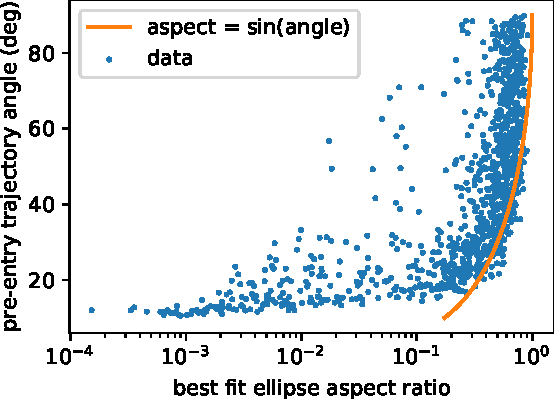
\includegraphics[width=0.45\textwidth]{figures/aspect_vs_angle}
    \caption{Aspect ratio vs initial trajectory angle. The orange line indicates the relationship proposed in \cite{daubar2019recently}.}
    \label{fig:aspect_vs_angle}
\end{figure}

Figure~\ref{fig:aspect_vs_angle} shows the connection between the two. We can see that, similar to what was proposed in \cite{daubar2019recently}, the dispersion is almost independent of $\theta$ for angles above $\sim$40 degrees.
For shallower angles however, the angle dominates other meteoroid features. This behaviour is what we would expect qualitatively; at steep angles, we expect the spatial distribution of craters to be dominated by random processes during the breakup events.
Indeed, our analysis shows that varying the RNG seed introduces relative variances of typically $~30\%$ if the other parameters are kept at a constant value.

\subsection{Dispersion}
The dispersion attempts to measure the total size of a cluster as seen on the photos.
A first idea for a measure might be the maximum distance between any two craters in a cluster.
Since this measure would be prone to outliers, \cite{daubar2019recently} suggested to instead consider the entire set of distances between all pairs of craters.
They then calculated the standard deviation of this set of distances.
In this work, we use the median distance. We found that it is often very similar to the standard deviation. Plus, it can also be defined for clusters with only two craters.

In our variable RNG seed analysis, we see that the dispersion is quite well defined for the two steeper trajectory angles (45 and 80 degrees). The relative error is between 10 - 15\%. At shallower angles, dispersion becomes significantly more variable with relative errors of $\sim$50\%. 

\begin{figure}[htbp]
    \centering
    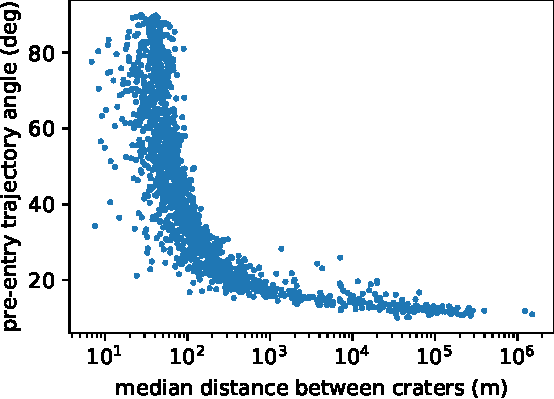
\includegraphics[width=0.45\textwidth]{figures/disp_vs_angle}
    \caption{Median dispersion vs. initial trajectory angle.}
    \label{fig:disp_vs_angle}
\end{figure}

For high values of dispersion, Figure~\ref{fig:disp_vs_angle} shows that in our model, the dispersion is largely influenced by the pre-entry impact angle. In fact, as figure~\ref{fig:disp_vs_aspect} shows, an important limitation of our model is that high levels of dispersion only occur for smaller aspect ratios.

Only considering one measure of the distribution of separation distances has its limitations however. In future work, we might want to consider additional features of this distribution. For example, the median or standard deviation does not capture sub-clustering of craters; that is, pockets of nearby craters that are clearly separated from the others.

\begin{figure}[htbp]
    \centering
    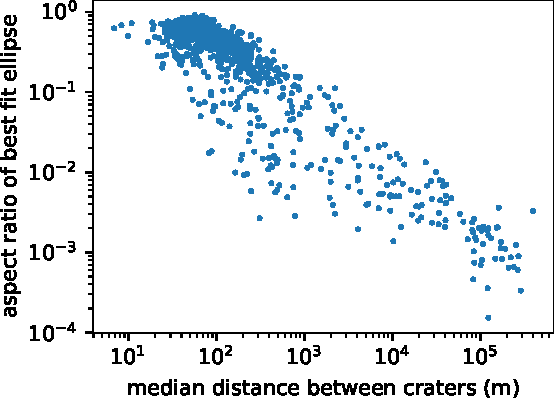
\includegraphics[width=0.45\textwidth]{figures/disp_vs_aspect}
    \caption{Median dispersion vs. aspect ratio of best-fit ellipse. It shows that there is a threshold for dispersion above which our model can only produce clusters with that value if they are distributed within a tight ellipse. For the model parameters we used, the threshold is about $100\unit{m}$.}
    \label{fig:disp_vs_aspect}
\end{figure}

\subsection{Number of craters}
The crater clusters mapped by \cite{daubar2019recently} only contain craters with a diameter of at least $1\unit{m}$, which is linked to the resolution of the images that they worked with.
Because of this limit, we would expect the number of craters large enough to be visible to provide a lower limit to the effective diameter, and therefore to the mass of the impactor, which is indeed what Fig.~\ref{fig:n_craters_vs_m} shows for clusters of more than 20 craters.
The number of craters generally varies by about 15 - 20\%.

\begin{figure}[htbp]
    \centering
    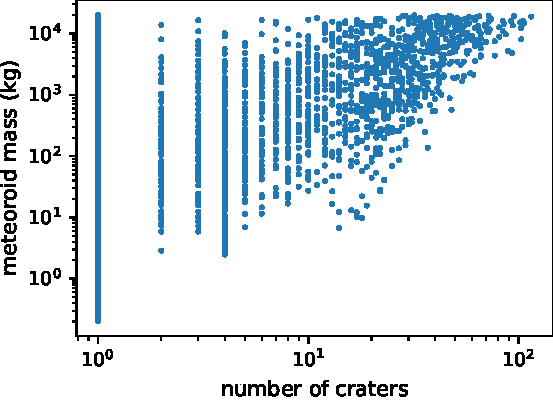
\includegraphics[width=0.45\textwidth]{figures/n_craters_vs_mass}
    \caption{Number of craters vs. initial meteoroid mass. Above about 20 craters, it provides a lower limit to the meteoroid mass. There is also a minimum mass to form at least two detectable craters.}
    \label{fig:n_craters_vs_m}
\end{figure}

\subsection{Fraction of large craters}
Considering this measure was proposed by \cite{newland2019CFM18}, who attempted to find a way to quantify the diameter-frequency distribution of craters in the clusters. The definition of a large crater is that its diameter $d_i$ has to be larger than a fraction $f$ of the largest diameter $d_\mathrm{max}$.
\begin{equation}
    f_\mathrm{large\,craters} = \left|\left\{d_i\ \big|\ d_i > f\cdot d_\mathrm{max}\right\}\right|
\end{equation}
\cite{newland2019CFM18} used $f = 0.5$ and were able to show that, with the inner structure in Table~\ref{tab:eric_inner_structure}, the fraction of large craters produced by the fragment-cloud model, at a given effective diameter, exhibits a similar distribution to the observational data \citep{daubar2019recently}. If they assumed a homogeneous inner structure however, this was decidedly not the case. It allowed them therefore to make a claim about the general inner structure of impactors on Mars.

In this work, we kept the inner structure fixed. We did not see an appreciable influence that fixing this quantity had on any of the meteoroid features.
Aside from an obvious one, where there is a minimum mass required to get a very small fraction of large craters (cf. fig.~\ref{fig:f_large_vs_mass}). This is what we would expect if there are one or two large craters; in order to form a sufficiently large number of small craters, a larger mass is required (Figure~\ref{fig:n_craters_vs_m}).

\begin{figure}[htbp]
    \centering
    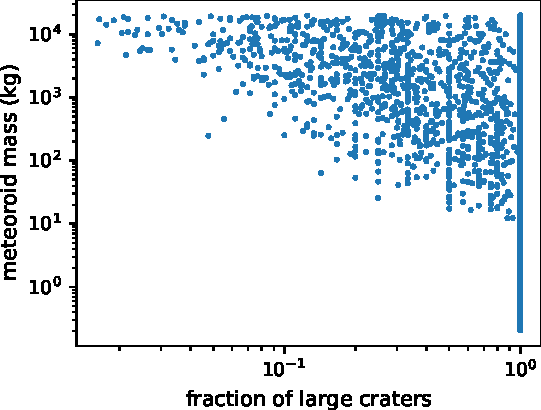
\includegraphics[width=0.45\textwidth]{figures/f_large_vs_mass}
    \caption{Number of craters vs. initial meteoroid mass. Above about 20 craters, it provides a lower limit to the meteoroid mass. There is also a minimum mass to form at least two detectable craters.}
    \label{fig:f_large_vs_mass}
\end{figure}

\subsection{Summary}

Table~\ref{tab:characteristics_summary} contains an overview of the findings presented above. We were able to show that there is no simple relationship by which meteoroid feature determines any characteristic of the crater cluster that it forms. We have identified two reasons for this. Even though many of these characteristics are defined in a way that should be rather resilient to outliers, our simulations show randomness in the breakup events of our model leads to significant variability.

Second, our Monte-Carlo simulation shows that a whole range of parameters can result in the same effective diameter for example.
But we have also found limits to this range of parameters. Only a limited range of combinations of mass, angle and core strength produce a similar number of craters and a similar effective diameter. For the dispersion and ellipse aspect ratio, both appear to be suitable indicators for impact angles shallower than 40 degrees.

It should therefore be possible to compute a distribution of meteoroid features that should be reasonably constrained in all features but velocity, which is what we investigate in the next section.

\begin{table*}
    \centering
    \begin{tabular}{l|c|c}
        & relative std deviation & significant parameters \\
        \hline
        $D_\mathrm{eff}$ & $\sim 1\%$ & mass, core strength, angle \\
        aspect & $\sim 30\%$ & angle \\
        dispersion & $\sim 10\%$ (steep $\theta$) - $\sim 60\%$ (shallow $\theta$) & angle \\
        $n$ craters & $ \sim 20\%$ & mass \\
        $f$ large craters & $\sim 30\%$& inner structure \citep{newland2019CFM18}, mass
    \end{tabular}
    \caption{Summary of findings on cluster characteristics}
    \label{tab:characteristics_summary}
\end{table*}
